\section{Recurrent Neural Networks}
So far we have considered only \textit{static} datasets: input and output don't have any time, any ordering or dependencies between each other.\\
(Aggiungere figura sequencernn)\\
The main idea is to think the input as a vector $X_i$ and consider a sequence of inputs in order to model that sequence of samples. 

Some relevant sequence are, for instance, time-series or text that, in general, are some sort of \textit{dynamical} data. To model this sequence you have different approaches: 
%So far input and output don't have time, do not have any ordering or dependences between each other.

%slide 3
%The idea is to think about the input as a vector and you have a sequence of input. We would like to go beyond the idea of having input and output and the model we are building is independent from the sequence of the samples , acutally we want to model the sequence of the samples. Some sequence relevant are time-series but also text. The idea is that we have a sequence of input and we would like to model this sequence. To model this sequence, you have different approach: 

\begin{itemize}
    \item \textbf{Memoryless} models: you don't explictly store a representation of the past, but you just use the previous $k$-samples to predict the next one
        \begin{itemize}
            \item  \textit{Autoregressive models}: predict the next input from previous ones using "delay taps"
            \item \textit{Feed Forward Neural Networks}: generalize autoregressive models using non-linear hidden layers. You feed your network with the $k$ past samples and you try to predict the next one. This approach is known as \textit{Sliding Window}        \end{itemize}{}
    \item \textbf{Memory-based} models: they are generative models with a real-valued hidden state which cannot be observed directly. The hidden state has some dynamics possibly affected by noise and produces the output. To compute the output the model has to infer hidden state. Input as treated as driving inputs.
        \begin{itemize}
            \item  \textit{Linear Dynamical System}: keep the state of the system which models the evolution of your data and define an output function which models the output given the current state of the system. In Linear Dynamical Systems the system becomes state continuous with Gaussian uncertaintly, transformations are assumed to be linear and the state can be estimated using \textit{Kalman Filtering}. One observation is that if you model your data in this way, you get a \textbf{stochastic} system. 
            \item \textit{Hidden Markov models}: you have a random variable which models the state of the system and another one that models the output of the system. The state is assumed to be discrete, state transitions are \textit{stochastic} (transition matrix). The output is a \textit{stochastic} function of hidden states. The states can be estimated via \textit{Viterbi algorithm}. In this model you do not have any input, but only a hidden state. This is a \textbf{stochastic} system
            \item  \textit{Recurrent Neural Network}: they are \textbf{deterministic} systems and they will be deepened more in the following chapters. 
        \end{itemize}{}
\end{itemize}{} 



%A model that is memory-less, you don't explicitly store a representation of the past but you just use the previous k-samples to predict the next one. This can be done with auto-regressive model or via feed-forward neural network. 

%(immagine appunti) To use a FNN to predict the next sample basing on the last two, you fed your network with the two inputs of the previous steps. You treat these two sample as input and you try to predict the next one. You don't need memory: this approach is know as Sliding Window. You don't necessary need memory to model time series. 

%You have also models with memory:
%Linear Dynamical systems: where you have a state of the system which model the evolution of your data and an output function which models the output given the current state of the system 

%Hidden Markov Model: evolution of the previous. You have a random variable which model the state of the system and another which models the output of the system

%Recurrent Neural Network: verranno approfondite

%slide 5 
%So in auto regressive model: you have a sequence of states, if the blocks represents the state or the output of the system at time zero, you try to predict one state looking k-step before.
%With FNN you generalize the classical linear model by having an hidden state. In this case, X2 is a function of x1 and x0 through an hidden state.

%slide 6
%If you want to do a change you have to add a state. For instance, you can have a model like this where your current input modify a state, your state impacts on the output. At the next time, the previous state is put forwarded, it is modified with the current input and generate the output, and so on and so forth, the state is put forward and so. The memory is hidden in the model and it is put forward while you do prediction.
%The idea is that you have some dynamics in the state and basically to compute the output you have to detect or estimate what is the current value of the state. If you have continuous state and linear transformation, it is basically linear Gaussian model and inferring the value of the state is what you do with a classical Kalman Filter. 
%One observation is that if you model your data in this way, you get a stochastic system.
%Another approach is the Hidden Markov model where you don't have the input, you have only an hidden state. 
%In neural network the things are more complex. 
%(so google presentation fare un'unica immagine con le varie figure alle slides 5-6-7 e mettere una label di quale modello si riferiscono)

\subsection{Recurrent Neural Networks}
Let's start modeling a standard system with a standard Feedforward Neural Network such as the one seen so far: the output is a non linear function of the weighted sum of the hidden neurons and these hidden neurons are a non linear function of the weighted sum of the input. \\ 
The classical way to add the memory is through \textit{Recurrent Hidden Neurons}, the blue ones in the Fig.\ref{wrap-fig:rnn}: a set of hidden neurons is added and their outputs are recurred. These hidden neurons have a feedback loop which makes their output depending on the previous value. \\
Memory via recurrent connections has some benefits:
\begin{itemize}
    \item Distributed hidden state allows to store a information efficiently
    \item Non-linear dynamics allows complex hidden state updates
\end{itemize}{}

\begin{wrapfigure}{l}{8.5cm}
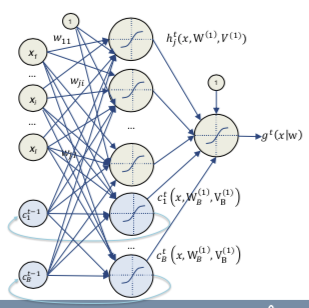
\includegraphics[width=8.5cm, height=7.2cm]{images/rnn.png}
\caption{Recurrent Neural Network}\label{wrap-fig:rnn}
\end{wrapfigure} 
 
These approach is due to Helmann and it is different from linear dynamical systems since one part of the hidden layer [the brown part] is \textit{time-less} and the other part is in charge of bringing forward the information. The blue part is a sort of summary of all the input that the network have seen so far. This summary is brought forward to the next step and it becomes non-linear combination of the previous state and the current input. \\
The blue nodes are also called \textit{c-nodes} because they provide the context to create the output.\\ \\
The context part of the network depends on the previous value of the context network and the current input which update the state: in fact, the \textit{context-neuron} is : 
%Adding the memory: the classical way the memory is added to a neural network is through recurrent hidden neurons(?). The most common way is to add a set of hidden neurons (the blue ones) and recur their outputs. These hidden neurons have a feedback loop which makes their output depending on the previous value. This is different from the linear dynamical system, since one part of the hidden layer (the brown part) is time-less and the other part (the blue) is in charge of bringing forward the information. You can image the blue part a sort of summary of all the input that the network have seen so far. This summary is brought forward to the next step, and the summary becomes non linear combination of the previous state and the current input. This model is due to Helmann. So you see the output depends also on the c-nodes. The c-nodes provides the context to provide the output. Context network depend on the previous value of the context network and the current input which update the state: in fact, the context-neuron is written as: 
$$
c_{\mathrm{B}}^{\mathrm{t}}\left(x, \mathrm{W}_{\mathrm{B}}^{(1)}, \mathrm{V}_{\mathrm{B}}^{(1)}\right)
$$
where $x$ is the input, $W_B$ are the weights from the input to the context network and $V_B$ are the weights from the context network to itself, so from the previous step to the current step.
In the figure there are other weights from $c_i^{t-1}$ to the brown neurons (from the context to the hidden) that can  be called $V$.\\
In general, the main formula of the RNN are shown below
$$
\begin{aligned}
g^{t}\left(x_{n} | w\right) &=g\left(\sum_{j=0}^{J} w_{1 j}^{(2)} \cdot h_{j}^{t}(\cdot)+\sum_{b=0}^{B} v_{1 b}^{(2)} \cdot c_{b}^{t}(\cdot)\right) \\
h_{j}^{t}(\cdot) &=h_{j}^{t}\left(\sum_{i=0}^{I} w_{j i}^{(1)} \cdot x_{i, n}+\sum_{b=0}^{B} v_{j b}^{(1)} \cdot c_{b}^{t-1}\right) \\
c_{b}^{t}(\cdot) &=c_{b}^{t}\left(\sum_{i=0}^{I} v_{b i}^{(1)} \cdot x_{i, n}+\sum_{b^{\prime}=0}^{B} v_{b b^{\prime}}^{(1)} \cdot c_{b^{\prime}}^{t-1}\right)
\end{aligned}
$$

%(immagine esempio appunti)

\begin{quote}
    \textit{"With enough neurons and time, RNNs can compute anything that can be computed by a computer}
\end{quote}{}

In 1990 there was a theorem that proves that if you have enough neurons and time, you can prove that this model is Turing-complete, as powerful as Turing machine.\\
This recurrent loop needs to be estimate: back-propagation needs that all the function %reverse
to be differentiable and the network to be feed-forward, but this architecture is not feed-forward anymore. So we have to modify back-propagation or find different algorithm to discover this loop. 

%Note: the different between rnn and hidden markov model or linear dynamical system is that, the latters are stochastic, this is deterministic: once you put an input, the output is always the same. It's non linear, complex but deterministic. 
If you want to consider the output at time t:
$$
g^{t}\left(x_{n} | w\right)=g\left(\sum_{j=0}^{l} w_{1 j}^{(2)} \cdot h_{j}^{t}(\cdot)+\sum_{b=0}^{B} v_{1 b}^{(2)} \cdot c_{b}^{t}(\cdot)\right)
$$
it is divided in two part, the forward and the recurrent respectively. We assume $B$ hidden neuron in the context part, $J$ are the neuron in the hidden state. \\
The context network is combination of previous values of the context network and the weighted sum of the input.\\ \\
%You can distinguish between forward and recurrent network. 
Instead, the \textbf{context update} is a non-linear function $c_b^t$ of the weighted sum of the previous context plus the linear combination of the current input. \\
We have more weights but not necessary in form of numbers but as a sort of weights, in the sense that the weights from the previous values of the memory state to the current value of the memory state are tricky to be defined because they represent the memory: these weights are the feedback loop.\\ 

But how to build the context part of the network? \\
%27:50
By definition, the previous %[version]
layer of the hidden state has the same number of  memory states because they are the same thing: basically, you have $B$ hidden neurons here in the context network [we are referring on the blue neurons on the right in Fig.\ref{wrap-fig:rnn}] and $B$ inputs which are the previous values of those hidden neurons, so the number of weights is $B*B$ and this is why you see here
$$
c_{b}^{t}(\cdot)=c_{b}^{t}\left(\sum_{i=0}^{I} v_{b i}^{(1)} \cdot x_{i, n}+\sum_{b^{\prime}=0}^{B} v_{b b^{\prime}}^{(1)} \cdot c_{b^{\prime}}^{t-1}\right)
$$
$b^{'}$ which goes from 0 to $B$ of the weights from $b^{'}$ to $B$.\\
This is a relevant part because we want to learn these weights via back-propagation, but while it's a reasonable standard back-propagation in the brown part, it's more tricky to have back-propagation in the blue part.\\ 

The trick is called \textbf{Back-propagation Through Time} and it is based on the following idea: \\
if the input $V_B^t$ is the output of the previous neuron, I can replicate this structure back in time and I can use the input $V_B^{t-1}$ to the previous neuron. So if the output at time $t$ is $
c_{B}^{t}\left(x, W_{B}^{(t)}, V_{B}^{(t)}\right)
$ , i.e. a combination of its previous value and the current input, I can replicate this node back.
%and now I have an output and I have an input which is the previous step to the (qualcosa). 
So you can back-propagate through these weights. Obviously to get the output you have to back-propagate again and again and again. \\
\begin{figure}
    \centering
    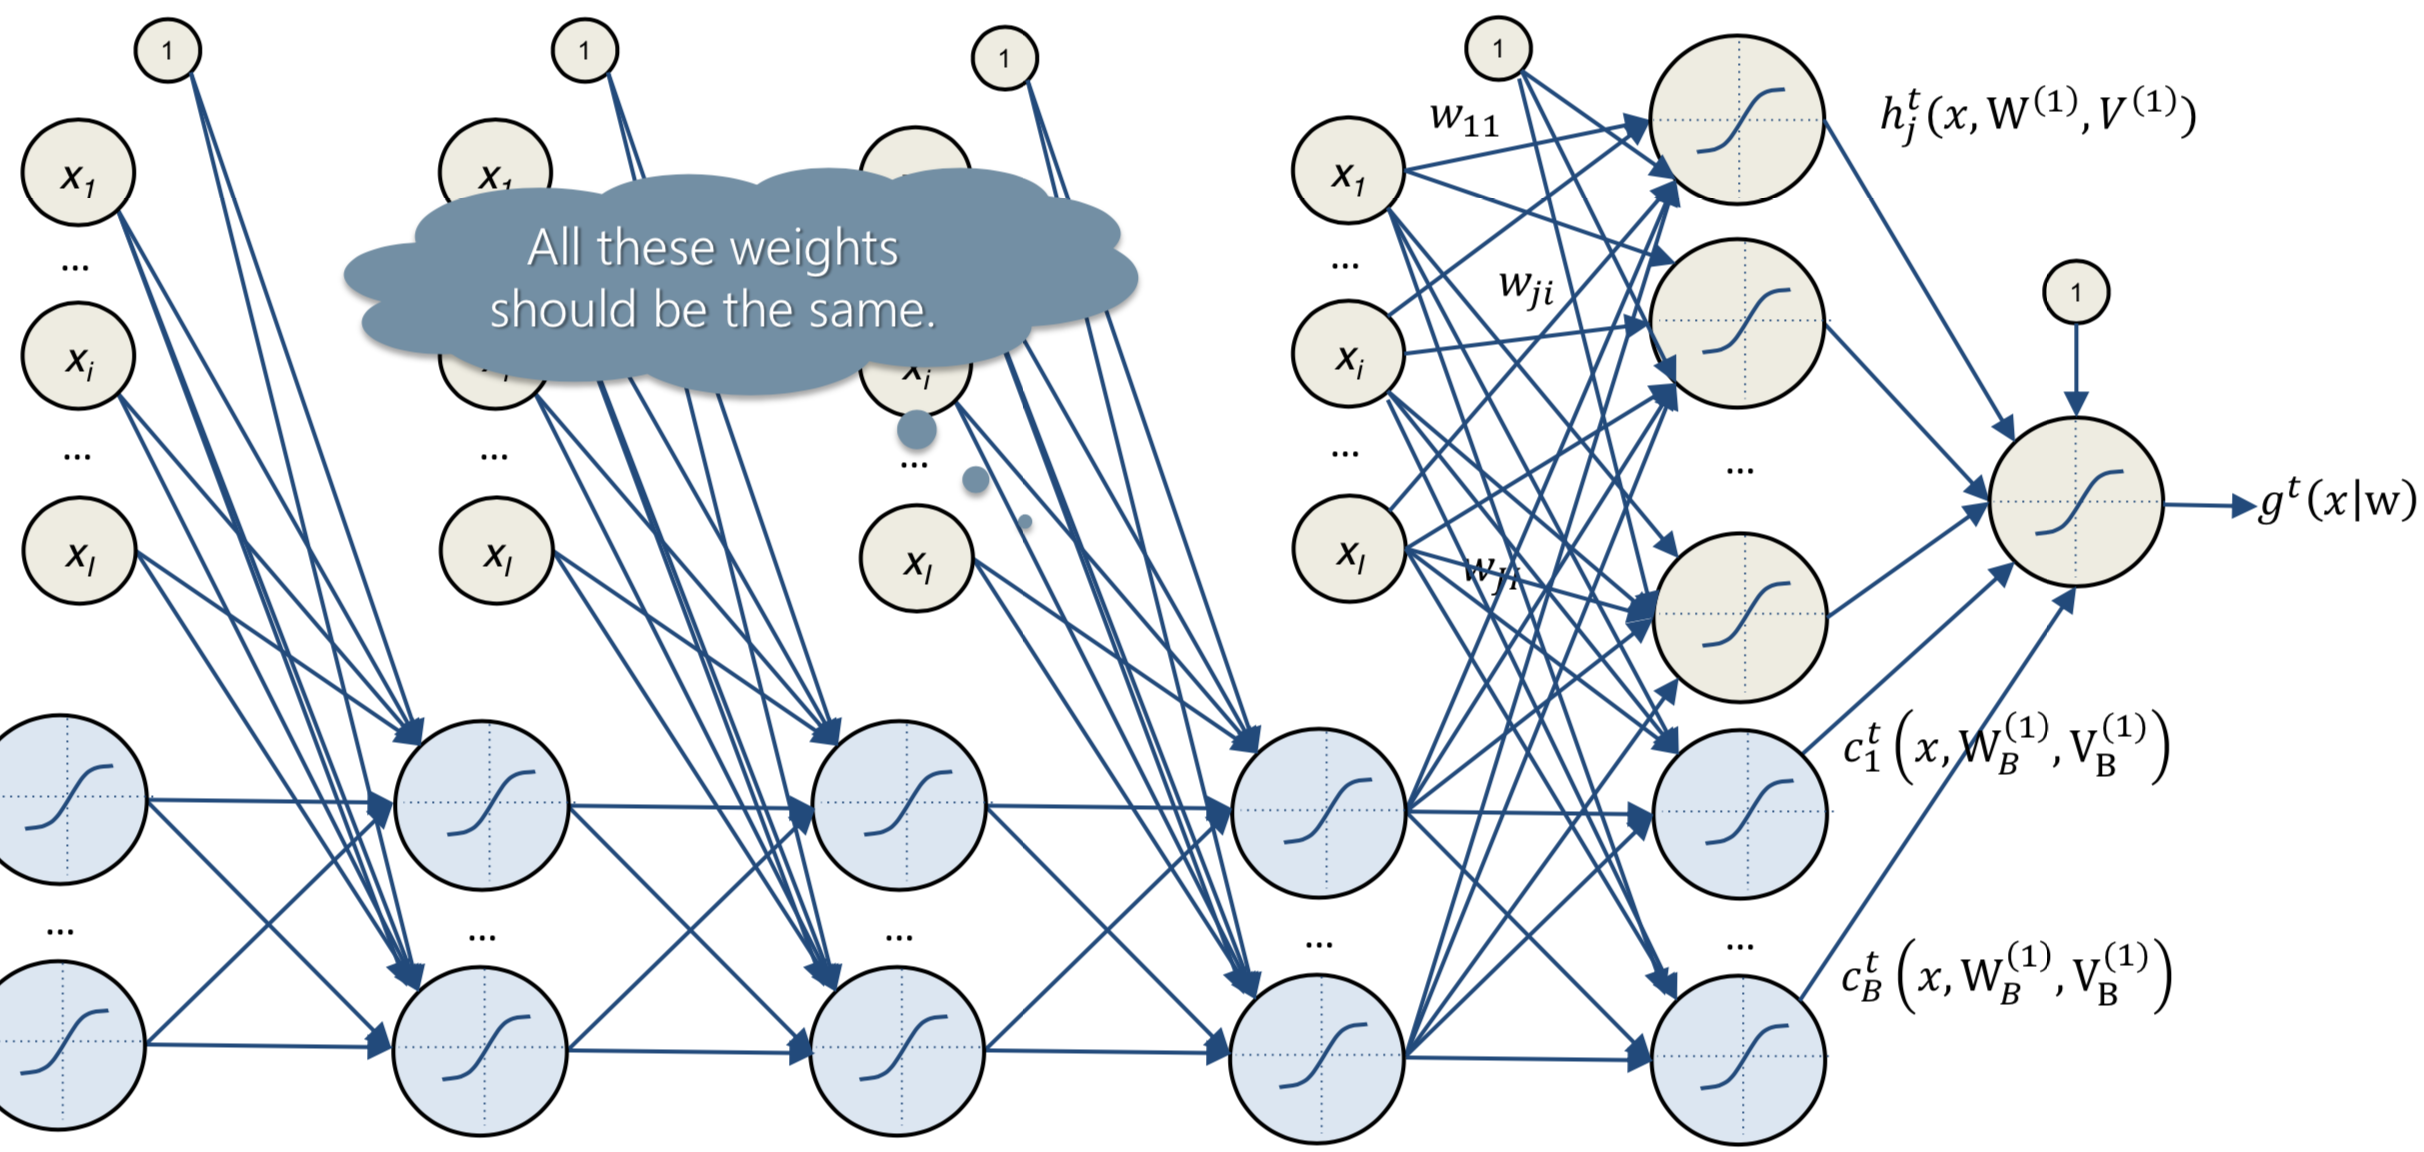
\includegraphics[width=15cm, height=7cm]{images/rnn_backpropagation.png}
    \caption{Backpropagation Through Time}
    \label{fig:rnn_back}
\end{figure}{}

The idea is to make multiple copies of the context network and associate weights to them, so you can back-propagate as a standard Feedforward Neural Network: it's standard because your dataset is finite so you do not need an infinitely long training sequence; if your training sequence has an hundred samples, you unroll for an hundred steps and you can back-propagate on that. \\
The problem is that this approach is not really sustainable for very long sequences, so you have to unroll until a certain point: this approach is called \textbf{Truncated Back-propagation}. This may look like limiting because you do not show, to the network, sequences longer than the limit imposed, but in practice it is not a limitation. \\ 
%Unrolling for 10 or 100 steps does not improve the performance of the model. 
One approach instead of doing full back-propagation can be to slice your dataset in chunks and unroll for the length of the chunks. So the idea is that you start from your loop and you unroll, then you get in principle a feedforward neural network. \\ 

%slide 11
Another important observation is that all the weights of the unrolled part must be the same through all the layers because if you run back-propagation in one neuron (such as the most right blue one), the gradient will be "the error x the derivatives x these weights x derivatives x the output of this neuron"; instead the gradient on the most left neuron %(credo)
is "derivative of the error x derivative of this x weights x derivative x weights x ... and so on (starting from the right to the left) x the output of this neuron". The two gradients %derivatives (forse intendeva i gradient?) 
are different because are computed via different formula. \\
The point is that if you unroll and you treat this "fake" feedforward neural network as classic feedforward neural network, you will end up with an inconsistency because all the weights should be equals %(non so di quali stia parlando)
$\rightarrow$ you have to implement back-propagation by forcing all these replicas to have the same value.\\
In practice, instead, works as follows:
\begin{itemize}
    \item Perform network unroll for $U$ steps
    \item Initialize $V,V_B$ matrices (all the replicas) to be the same. The trick is here, to keep them equal, initialize them equal.
    \item Compute gradients, but you update using the average gradient of all the copies, so you update replicas with the average of their gradients
    $$
    V=V-\eta \cdot \frac{1}{U} \sum_{0}^{U-1} \frac{\partial E}{\partial V^{t-u}}  \quad V_{B}=V_{B}-\eta \cdot \frac{1}{U} \sum_{0}^{U-1} \frac{\partial E}{\partial V_{B}^{t-u}}
    $$
\end{itemize}
There are two ways to perform this pipeline:
\begin{enumerate}
    \item Unroll $\rightarrow$ Compute Gradient  $\rightarrow$ Update all the weights independently  $\rightarrow$ Compute the Average Gradient
    \item Unroll  $\rightarrow$ Compute Gradient  $\rightarrow$ Update all the weights with the Average Gradient
\end{enumerate}{}

%by unfolding the network for $U$ steps, then  initialize at the beginning the $V,V_B$ matrices at some value and copy this initialization. The trick that keep them equal is initialize them equal. This works also for the other V matrix and also for $W_b$ matrix entering this node. Then you compute all the gradients, but when you update these matrix, you update using the average gradient of all the copies. Basically, you make a step of gradient descent on this $V_B$ as follows: 
%$$
%V_{B}=V_{B}-\eta \cdot \frac{1}{U} \sum_{0}^{U-1} V_{B}^{t-1}
%$$

%Doing this, you update each matrix with its own gradient and then you can average from this [?].
%There are two ways of performing this: 
%First: you unroll, compute gradient, update all the weights independently and compute the average 
%Second: you unroll, compute the gradient and update with the average gradient. 

With this trick we are forcing all the replicas to have the same weights. It's a sort of weights sharing. \\ 

%If we unfold (credo sia uguale a unroll), you can compute the gradient

How do you initialize this? 
\begin{itemize}
    \item First approach: initialize to 0
    \item Second approach: learn how to initialize. Take the most back-in-time [blue] node as the first value of the state, so you can learn what is its value: instead of differentiating with respect to this weight, you differentiate w.r.t. that node. By doing this you train the sequence to learn what should be the initial state that works best. 
\end{itemize}{}
%One trick is to learn also the initial state: when you start the network, when you get the first input, you see the output depends on the previous step, but the previous step is not defined with the previous input. So you can set it to 0. Another approach, you can threat the last of the nodes (il nodo blu più a sinistra) as the first value of the state, so you can learn what is its value: instead of differentiating with respect to this weight, you differentiate w.r.t. that node. By doing this you train the sequence to learn what should be the initial state that works best. 

How long we can go back in time? \\
Sometimes output might be related to some input happened quite long before. However, back-propagation through time was not able to train recurrent neural networks significantly back in time because it is not able to back-propagate through many layers. \\ \\
It is a problem mainly due to text analysis. They find out that there is no way to store more than 10-20 steps or in other term there is no way to learn with network unrolling a window longer than few dozen of terms. \\ 

The reason is due to \textbf{Vanishing Gradient}: if you think about network unrolling for a very long series of time, what happens is that the gradient will be the product of the derivatives of all the intermediate functions and will get to zero.\\
Usually the initialization of the network is random and there is no way to move the memory of the initial steps (the blue top left neurons) anywhere with respect to the initial initialization. So the memory of this model is random since it is not possible to use inputs from the past. \\ 

%slide 14
To better understand why it is not working, consider a simplified case: \\ \\
\vspace{0.2cm}
\begin{minipage}{\linewidth}
        \centering
        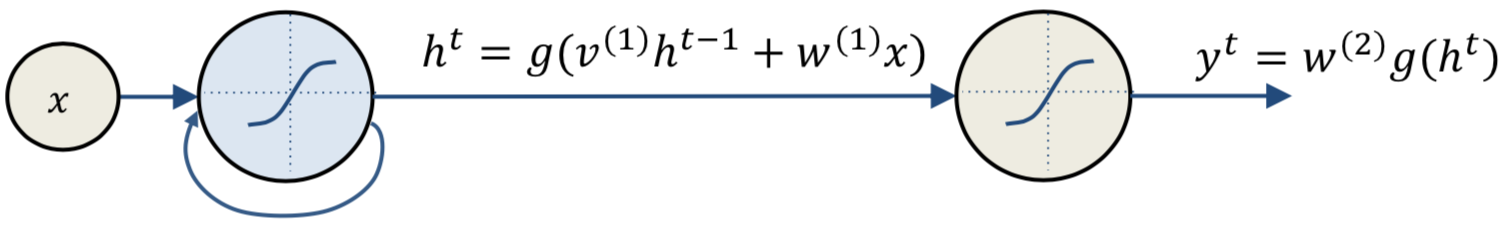
\includegraphics[width=15cm]{images/simplified_rnn.png}
        \label{fig:sim_rnn}
\end{minipage}
\vspace{0.2cm}

The model represented is a simplified model. Considering $v^{(1)}$, it is how much the output of this neuron is weighted to compute the next one.  The output of the hidden neuron is a non-linear function g() depending on the weighted sum of the previous loop $v * h^{t-1}$ plus a weighted input. %Then you have an output neuron. 
Focusing on the first part of the network, assume you want to derive the error w.r.t. input weight %this weight (quello dell'input) 
and you want to minimize the sum over all the sequences of the derivative of the error at time t w.r.t. to the weight of the input. This weight appears in the input but also in the previous inputs. So this derivative is not so easy, but we can use the trick of the chain rule of derivatives: 
%consider the sum over all possible sequences; take one of this sequence and find what is the error at time t w.r.t. the weights. This derivative is equal to the sum over all timestamps of the derivative wrt to the previous output, the derivative of the output w.r.t. to the input which is h at time t, times the derivative of this w.r.t the previous hidden value, times the derivative of it times the derivative value w.r.t. x (penso abbia guardato la figura più che la formula delle derivate). 
$$
\frac{\partial E}{\partial w}=\sum_{t=1}^{S}\left(\frac{\partial E^{t}}{\partial w}\right) \rightarrow {\frac{\partial E^t}{\partial w}} = \sum_{t=1}^{t} \frac{\partial E^t}{\partial y^t} \frac{\partial y^t}{\partial h^t} \frac{\partial h^t}{\partial h^k} \frac{\partial h^k}{\partial w}
$$
So basically, depending on how much is k, you derive w.r.t. to one of the past loops. If you look at the second formula, you notice that the derivative of the hidden neuron output w.r.t. any of the output in the past,  is $$
\frac{\partial h^{t}}{\partial h^{k}}=\prod_{t=k+1}^{t} \frac{\partial h_{i}}{\partial h_{i-1}}=\prod_{i=k+1}^{t} v^{(1)} g^{\prime}\left(h^{i-1}\right)
$$
i.e. the product of the derivatives from $k$ to $t$ of the derivative of time $t$ over $t-1$: 
%(guardare gli appunti per un esempio di questa parte)
%If you define the derivative as g'(), you see that this derivative is the product of:
%$$
%\frac{\partial h^{t}}{\partial h^{k}}=\prod_{i=k+1}^{t} \frac{\partial h_{i}}{\partial h_{i-1}}=\prod_{i=k+1}^{t} v^{(1)} g^{\prime}\left(h^{i-1}\right)
%$$
Note that the derivative of $g(v()*h)$ is $g^{\prime}()* v^{(1)}()$. %Non ne sono sicuro di quest'ultima frase
Considering the norm
$$
\left\|\frac{\partial h_{i}}{\partial h_{i-1}}\right\|=\left\|v^{(1)}\right\|\left\|g^{\prime}\left(h^{i-1}\right)\right\| \Rightarrow\left\|\frac{\partial h^{t}}{\partial h^{k}}\right\| \leq\left(\gamma_{v} \cdot \gamma_{g^{\prime}}\right)^{t-k}
$$
It means that the the norm is less or equal than the product of two terms: $\gamma_v$ is given by the weights, the other  $\gamma_{g^{\prime}}$ is given by the derivatives, and the exponent is how long is the past. \\
So if you go one step back, you see that this is the v*derivative, if you go 2 step back you have the product v derivatives * v*derivative: depending of the value of this term, you have a sequence of products which might go either to infinite or zerO. \\
In particular, if 
%(credo intenda la norma di delta $h^t$ fratto delta $h_k$)
$$ \rho = \left\|\frac{\partial h^{t}}{\partial h^{k}}\right\| < 1$$
%is less than 1, 
it converges to zero.
%because it is a number which is less then 1. 
%This is the gradient of the error at time $t$ wrt the weights,  the contribution of past inputs goes to zero.
If the derivative is less than 1, the gradient of the error function w.r.t. to an input $t-k$ steps back in the past goes to 0. \\
The point is that if you try to update the weight of an input $k$ epochs ago, your gradient is null. If you use for this weight either a \textit{tanh} or a \textit{sigmoid}, by definition $\gamma_{g^{\prime}}$ is less than 1. We have seen that the derivative of sigmoid and tanh, are respectively, $0.5$ or $0.25$: it means that in few steps in the past, the derivative of the output w.r.t. to the input will be 0 $\rightarrow$ With Sigmoids and Tanh we have Vanishing Gradient. \\
You may think that the other number $\gamma_{v}$ is going to compensate, but it means the more you go in the past, the more it should be bigger, but it make no sense: this value $\gamma_{v}$ is a constant. If it is a big constant such that the product is bigger than 1, it worst because you have that
%(norma di delta $h^t$ fratto delta $h_k$)
$\rho > 1$
%is greater than 1 to the 3 hundred-twenty, 
so the gradient will explode numerically. \\

%slide 15
The only solution is to force all gradient to be either 0 or 1, otherwise vanishing gradient or gradient explosion occur. 
The only way to perform is using \textbf{ReLu}: 
$$g(a) = ReLu(a) = max(0,a) \Rightarrow g^{\prime (a)} = 1_{a>0}$$ 

%The only possible value to set to this in order to not explode is 1, so you have to force for this loop the derivative of wrt the loop = 1, otherwise this term is greater than 1 explode, if less it vanishes. To force this loop to have derivative 1, since this loop is the derivative of the activation function, if you have an activation function for which the derivative is 1, you guarantee that you don't have vanishing gradient due to this step. You have to use ReLu. This not resolve the exploding gradient problem but if you initialize the weight small enough, the gradient will try to fit them without getting an explosion. 
This solve part of the story, no more vanishing gradient, but you have still the risk of exploding gradient. \\
If we force this loop to have weight = 1, we guarantee nor exploding or vanishing gradient because the derivative w.r.t. to the previous step will be always 1.\\
It is constraining the model by solving the vanishing gradient and the exploding gradient. By doing this you make the output dependent on whatever time you want. It is like a shortcut connection with all timestamps in the past.\\ \\
If you look closer, if the weight $v^{(1)}$ is = 1, you do not need to train the model; now this is a pure Feedforward Neural Network with all previous steps. This weight has not to be trained, for all those replicas you know already the weights, they are all 1, so no training is require for this loop.\\
This kind of object is called \textbf{Constant Error Carousel}.\\ By doing this the output depends on all the history of the input. The problem of the network is that it can \textit{only accumulate the input}, it just computes the integral of the input. \\This topology is useless because it is only integrating the input. 

%1:06:50
\subsubsection{Long-Short Term Memories}
Hochreiter \& Schmidhuber (1997) solved the problem of vanishing gradient designing a memory cell using logistic and linear units with multiplicative interactions. \\

\begin{wrapfigure}{l}{7cm}
    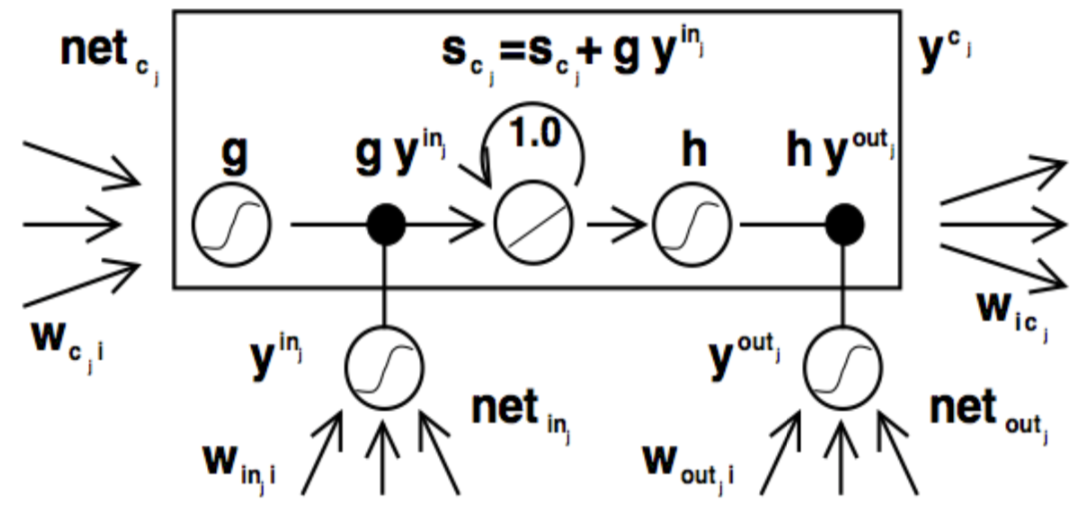
\includegraphics[width=7cm]{images/lstm_original.png}
    %\label{fig:lstm_org}
\end{wrapfigure} 

The creators started from the idea of Constant Error Carousel (CEC) and they thinks that now that we have an accumulator of the input, the only things to do is to build a network to learn when it is worth to add an input to the memory and when it is worth to read an input from the memory. \\ \\
The idea is to have some of \textit{gate} mechanism where:
\begin{itemize}
    \item[--] Information gets into the cell whenever its \textit{“write”} gate is on.
    \item[--] The information stays in the cell so long as its \textit{“keep”} gate is on.
    \item[--] Information is read from the cell by turning on its \textit{“read”} gate.
\end{itemize}{}
The gates are based on Constant Error Carousel. You can back-propagate through this since the loop has fixed weight. 

%To get out of the above issue,  is the idea of LSTM where the creators started from the idea of Constant Error Carousel and they said ok, now I have this CEC cell which is able to accumulate the input, what the network need to learn is when it is worth to add an input to the memory and when it is worth to read an input from the memory. The idea is to have some gating mechanism where you have this CEC, and you have a neural network which decides when it is useful to write in this memory and another network that decides when cancel or erase the memory and another network which decides when it is time to read from the memory.
Decision (e.g. as write/not-write) are based on the output of a Sigmoid; instead, the loop is ruled by a ReLu activation function. This kind of cell is the first \textbf{Long-Short Term Memories} idea. \\
The current architecture of the cell is shown below:

\vspace{0.2cm}
\begin{minipage}{\linewidth}
    \centering
    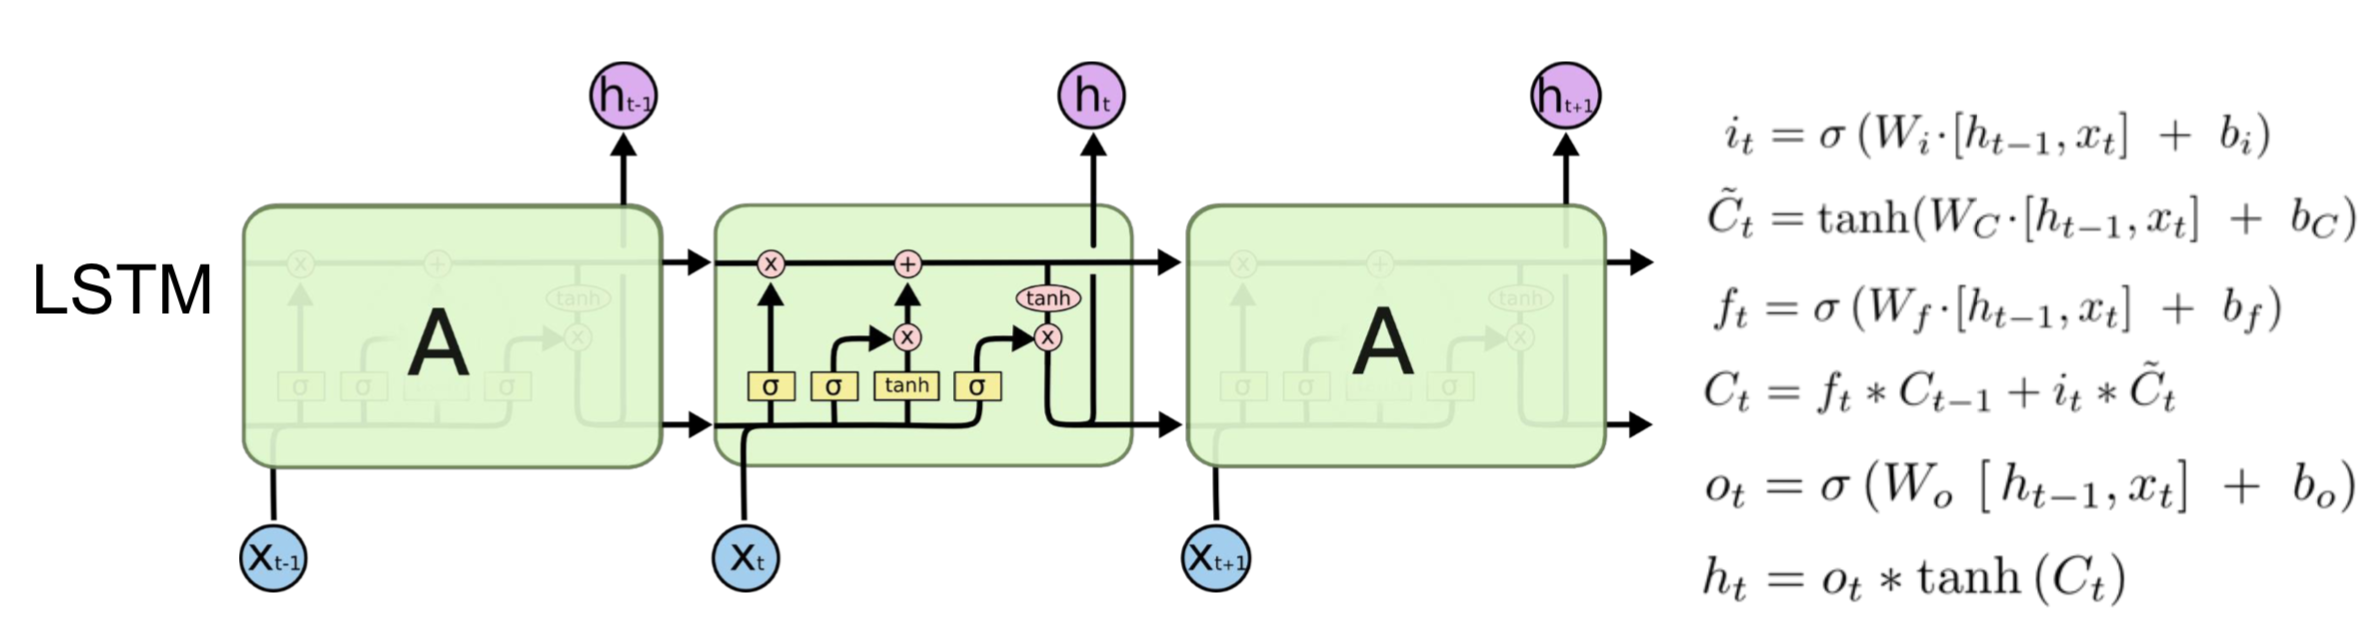
\includegraphics[width=15cm, height=4.5cm]{images/lstm.png}
    \label{fig:lstm}
    % \captionof{LSTM}
\end{minipage}
\vspace{0.2cm}

%This network [quella più a sinistra $net c_j$]  (in realtà penso più i gate che fanno accedere alla cella) have sigmoidal activation function which if says 0 you don't add anything in the memory, if 1 you add to the memory. The other network $net in_j$ decides what to add (+1 or -1), so these two modulate the content of the memory, based on the input: basing on the input it decides if store or not to or, if erase or not the memory.
%Nel mezzo c'è la Relu function which is a linear function, with the loop. Then there is the output of the network.
%Assume you have many of these cell and you output may depend on some of those. This cell is the first LSTM idea. 

%The nice thing is that you don't need unrolling because you can put many of these in the sequence and you can train without network unrolling because you don't need to train the weigth of the constant error carousel. 

%slide 17
%This is the architecture of RNN where at time t, the output of your network is a function of your current input and of your previous state. 

%slide 18
Different gates are highlighted:
\begin{itemize}
    \item[--] Input gate: the input is computed by the $tanh$ path and it is multiplied by this $sigmoidal$ part. It states if it is worth or not to write in the memory
    \item[--] Forget gate: in charge of re-writing or erasing the content of the memory. The memory is multiplied by a $sigmoid$, which indicates to keep the input if the sigmoid is equal to 1, otherwise erase the memory before adding the input. 
    \item[--] Memory gate: decide on adding the input to the previous state of your network. The memory is the sum of the forget gate and the input gate. 
    \item[--] Output gate: it is the combination of tanh and the reading mechanism controlled by a sigmoid. 
\end{itemize}{}

With LSTM networks you can build a computation graph with continuous transformation: the idea is that you can build an internal representation of the history of the input. This internal representation is updated at each input. \\
We can build different configurations of LSTM: 
\begin{itemize}
    \item One-to-One: translate one to one, one input and you want to translate it in another. For each input you predict one output
    \item One-to-many: one input and you want to predict many output. If x is the input, the idea is that the input modifies the state of the network and what happens is that you output one value, then another one, then another one. This kind of approach is used in Captioning: you enter an input (an image), you start with the first word, the you feed the model with this first word and you output the second word and so on; you write textual description for a single input. 
    \item Many-to-one: sequence of input and you want one output: example is Text Classification. 
    \item Many-to-many: it is in Video Classification or Video Captioning.
    \item Sequence-to-Sequence: you enter a sequence, then you have a state and the machine is started with this state. Then you generate a sequence. You think this kind of network as a sequence encoder. Since this model can be used also for generation, you have an input sequence and you use the state of this machine to generate a new sequence. This is the way most of text prediction and question answer are trained: you have a sequence encoder; once encoded this hidden representation for the sentence, you use a decoder (which is the same or a different LSTM) which is trained to output sequence conditioned on the value of this state. 
\end{itemize}{}

%Yo have different gates: 
%input gate: get the input
%the memory gate: you decide to add to the previous state of your network the input. The memory is the sum of the forget gate and the input gate

%The input is computed by the tanh path and it is multiplied by this sigmoidal part which says if it is worth or not to write in the memory

%Forget gate: in charge of rewriting or canceling the content of the memory. Decides whether it is worth to keep or decrease the content of the memory: you see that the memory is muliplied by a sigmoid which indicates to keep the input if the sigmoid is equal to 1, otherwise erase the memory before adding the input. 
%[Penso che i sigma siano i gate che sono fatti proprio da sigmoid function]

%Output gate is combined with some tanh and there is the reading mechanism which is this sigmoid multiplied by the gate.

%There is this forget gate: this network could learn to forget, but in order to do this it has to learn to remove content from the memory. So in the current implementation of LSTM, the forget gate is in charge of erasing partially the content of the network. 

\subsubsection{Gated Recurrent Unit}
An evolution of this memory is the \textbf{Gated Recurrent Unit}. It is more or less the same of LSTM: it combines the forget and input gates into a single "update gate". It also merges the cell state and hidden state, and makes some other changes.

%slide 24
%What can you do with LSTM: the idea is that they can build an internal representation of the history of the input. This internal representation is updated at each input. 
%At the beginning, we have this representation (slide24), you have an input, some hidden representation and the output is a function of this hidden representation. Then another input modifies the hidden layer and so on. 

%slide 25
%Se coloriamo le varie parti, we can build some different configuration of LSTM: 
%slide 26
%You can have mulitple LSTM layers. You have the input, then one LSTM which create a low level memory of the input, then another LSTM which remember an High level representation of the input, then you can have a non-linear function of the hidden layer as the output of the model

\subsection{Tips and Tricks}
Sometimes you can use \textbf{bidirectional LSTM}: if you have for instance many-to-one approach, you can read the sequence from left to right and vice-versa, put the two encoding together and classify the output with it. This is used often if you have to predict the output only having seen the entire sequence: you can process the sequence in the two direction. You cannot do it always, if you predict online, you cannot use it. \\

Another trick is in weight initialization:
\begin{itemize}
    \item Could initialize them to a fixed value
    \item Better to treat the initial state as learned parameters:
        \begin{enumerate}
            \item Start off with random guesses of the initial state values
            \item Backpropagate the prediction error through time all the way to the initial state values and compute the gradient of the error with respect to these
            \item Update these parameters by gradient descent
        \end{enumerate}{}
\end{itemize}

%you have to initialize the state of the network to a given state. One possible way is to initialize to an fixed value. It can be interest when you learn the network, to learn also the initial state of the network.